\subsection{Unit testing cho các thành phần logic backend}

Unit testing là bước đầu tiên và quan trọng nhất trong chiến lược kiểm thử đa tầng, tập trung vào việc xác minh tính đúng đắn của các "tế bào" nghiệp vụ nhỏ nhất trong hệ thống Backend. Tại đây, các phương thức xử lý logic, các quy tắc tính toán và các ràng buộc dữ liệu được kiểm tra một cách độc lập, tách biệt hoàn toàn với cơ sở dữ liệu, hệ thống tin nhắn hay các dịch vụ ngoại vi khác.

\subsubsection{A. Chiến lược và mô hình kiểm thử}

Nhờ kiến trúc phân lớp rõ ràng và khả năng tiêm phụ thuộc của Spring Boot, việc thực hiện kiểm thử đơn vị cho các dịch vụ nghiệp vụ trở nên thuận tiện và hiệu quả. Nhóm sử dụng khung làm việc JUnit 5 kết hợp cùng thư viện Mockito để cô lập hoàn toàn lớp logic cần kiểm thử khỏi các thành phần ngoại vi như Database hay các dịch vụ khác.

Trong hệ thống, tầng service đóng vai trò là "bộ não" điều khiển toàn bộ luồng nghiệp vụ. Do đó, kiểm thử đơn vị tại đây được thực hiện theo chiến lược White-box Testing, tập trung vào cấu trúc mã nguồn và tính chính xác của các thuật toán xử lý.

Để đảm bảo các bài thử nghiệm có tính cấu trúc và dễ bảo trì, nhóm áp dụng chặt chẽ mô hình Arrange – Act – Assert (AAA):

\begin{itemize}
    \item Arrage: Đây là giai đoạn chuẩn bị ngữ cảnh cho bài test. Nhóm sử dụng annotation @Mock để tạo ra các đối tượng giả lập cho repository, kafka producer hoặc các feign client. Các dữ liệu mẫu được khởi tạo và định nghĩa hành vi thông qua Mockito.when(...).thenReturn(...).
    \item Act: Gọi phương thức nghiệp vụ cụ thể trong service cần kiểm tra với các tham số đã chuẩn bị. Đây là bước kích hoạt logic lõi của hệ thống.
    \item Assert: Sử dụng các hàm Assertions như assertEquals, assertNotNull, assertThrows để đối chiếu kết quả thực tế với kỳ vọng. Đồng thời, nhóm sử dụng Mockito.verify() để xác nhận các tương tác với các thành phần phụ thuộc như việc lưu dữ liệu vào DB hay gửi tin nhắn qua Kafka, có diễn ra đúng như thiết kế hay không.
\end{itemize}

\subsubsection{B. Công cụ thực hiện chuyên sâu}

Nhóm sử dụng bộ công cụ tiêu chuẩn công nghiệp trong hệ sinh thái Java Spring Boot:

\begin{itemize}
    \item JUnit 5 (Jupiter): Cung cấp các Annotation điều khiển luồng test như @BeforeEach, @AfterEach và các câu lệnh khẳng định mạnh mẽ.
    \item Thư viện then chốt để thực hiện kỹ thuật Isolation Testing. Nhờ Mockito, nhóm có thể kiểm tra logic của một Service mà không cần khởi chạy toàn bộ Application Context, giúp tốc độ thực thi test chỉ tính bằng mili giây.
    \item Được tích hợp để tăng khả năng đọc hiểu của mã nguồn kiểm thử thông qua các câu lệnh dạng chuỗi, giúp việc so sánh các đối tượng phức tạp như danh sách sản phẩm trở nên trực quan hơn.
\end{itemize}

\subsubsection{C. Phân loại và các kịch bản kiểm thử tiêu biểu}

Các kịch bản kiểm thử được chia thành ba nhóm chính để bao phủ toàn bộ các khả năng có thể xảy ra trong thực tế:

\begin{itemize}
    \item Nhóm kịch bản thành công: Xác nhận hệ thống hoạt động đúng khi mọi điều kiện đầu vào đều lý tưởng.
    \item Nhóm kịch bản biên và điều kiện logic: Kiểm tra các tình huống nhạy cảm hoặc dữ liệu nằm ở ngưỡng giới hạn.
    \item Nhóm kịch bản xử lý ngoại lệ: Xác minh khả năng "tự vệ" của hệ thống trước dữ liệu sai lệch hoặc vi phạm quy tắc nghiệp vụ.
\end{itemize}

\begin{figure}[H]
    \centering
    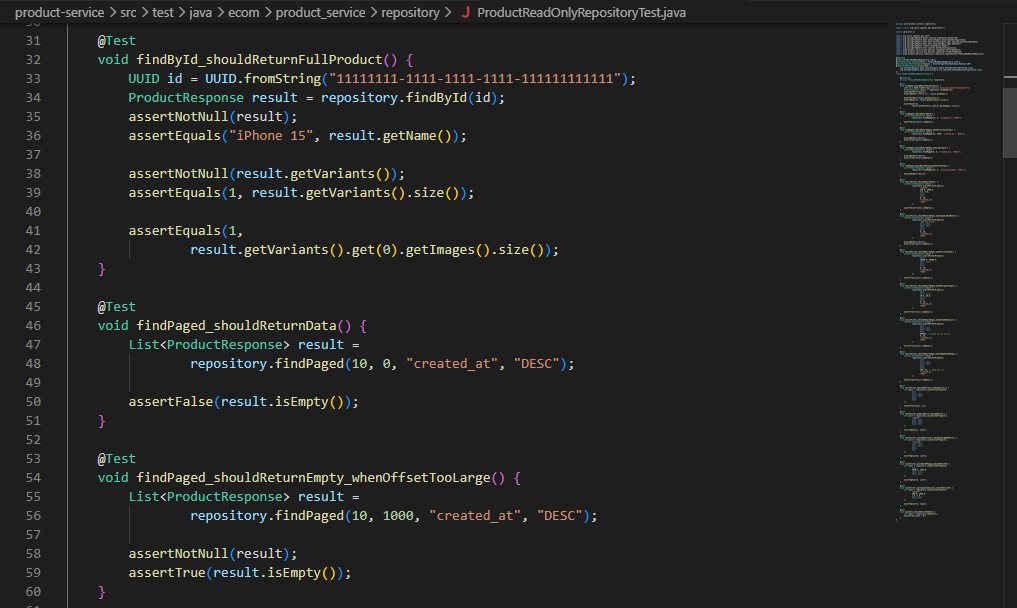
\includegraphics[width=0.9\linewidth]{images/chap8/happy-path-1.PNG}
    \vspace{0.7cm}
    \caption{Các kịch bản kiểm thử thuộc nhóm thành công trong ProductReadOnlyRepositoryTest}
    \label{fig:happy-path-product-repo}
\end{figure}
Hình \ref{fig:happy-path-product-repo} minh họa một số kịch bản kiểm thử tiêu biểu thuộc nhóm kịch bản thành công. Cụ thể, các phương thức như \texttt{findById\_shouldReturnFullProduct} và \texttt{findPaged\_shouldReturnData} xác nhận rằng hệ thống có thể truy vấn và trả về dữ liệu chính xác khi các tham số đầu vào hợp lệ và dữ liệu tồn tại trong cơ sở dữ liệu. Trong đó, kịch bản \texttt{findById} kiểm tra việc trả về đầy đủ thông tin của một sản phẩm, bao gồm các biến thể và hình ảnh liên quan, thể hiện tính toàn vẹn của dữ liệu. Đồng thời, kịch bản \texttt{findPaged} đảm bảo chức năng phân trang hoạt động đúng, trả về danh sách sản phẩm không rỗng khi tham số phân trang hợp lệ. Những kiểm thử này đóng vai trò quan trọng trong việc xác nhận các luồng chức năng chính của hệ thống hoạt động đúng như kỳ vọng trong điều kiện lý tưởng.

Tiếp theo, các Hình \ref{fig:edge-case-min-order} và Hình \ref{fig:edge-case-capping} đại diện cho nhóm kịch bản biên và điều kiện logic, tập trung vào việc xác minh các ràng buộc nghiệp vụ phức tạp của hệ thống.
\begin{figure}[H]
    \centering
    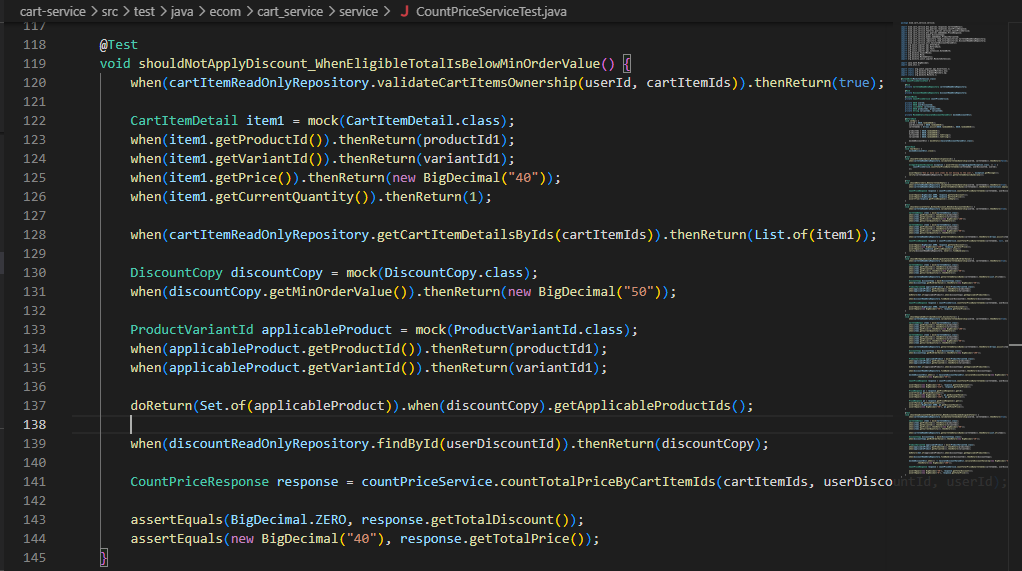
\includegraphics[width=0.9\linewidth]{images/chap8/edge-case-1.PNG}
    \vspace{0.7cm}
    \caption{Kiểm tra điều kiện ngưỡng giá trị đơn hàng tối thiểu trong CountPriceServiceTest}
    \label{fig:edge-case-min-order}
\end{figure}

Hình \ref{fig:edge-case-min-order} minh họa kịch bản kiểm thử một trong những quy tắc nghiệp vụ quan trọng nhất của hệ thống giảm giá: điều kiện về giá trị đơn hàng tối thiểu. Trong trường hợp này, dữ liệu kiểm thử được thiết lập với tổng giá trị sản phẩm hợp lệ chỉ đạt 40 đơn vị, trong khi mã giảm giá yêu cầu ngưỡng tối thiểu là 50 đơn vị. Kết quả kiểm chứng qua các câu lệnh \texttt{assertEquals} xác nhận rằng mức giảm giá thực tế trả về bằng 0 và tổng giá trị đơn hàng được giữ nguyên. Điều này khẳng định hệ thống có khả năng kiểm soát chính xác các điều kiện ràng buộc, đảm bảo các chương trình khuyến mãi chỉ được kích hoạt khi người dùng thỏa mãn đầy đủ các tiêu chí kinh doanh đã đề ra.

Bên cạnh đó, Hình \ref{fig:edge-case-capping} trình bày kịch bản biên giả lập tình huống mức giảm giá tính toán được (100 đơn vị) vượt quá tổng giá trị của các sản phẩm có thể áp dụng giảm giá (50 đơn vị). Thông qua việc giả lập hành vi của \texttt{CaculateDiscountValueUtil}, kết quả cho thấy hệ thống đã thực hiện "chốt chặn" mức giảm giá tối đa bằng đúng giá trị sản phẩm, dẫn đến giá sau giảm không bị âm. Việc kiểm tra này không chỉ đảm bảo tính ổn định của thuật toán tính toán mà còn ngăn chặn các rủi ro về sai lệch dữ liệu tiền tệ trong các tình huống cấu hình giảm giá cực đoan.
\begin{figure}[H]
    \centering
    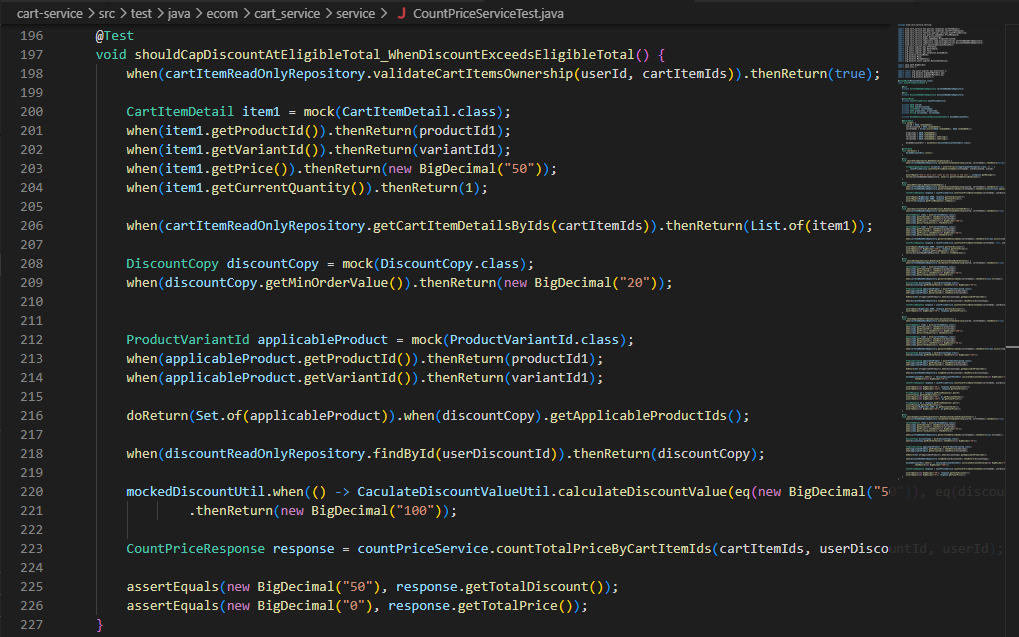
\includegraphics[width=0.9\linewidth]{images/chap8/edge-case-2.PNG}
    \vspace{0.7cm}
    \caption{Kịch bản kiểm thử giới hạn mức giảm giá tối đa }
    \label{fig:edge-case-capping}
\end{figure}

Cuối cùng, để hoàn thiện chiến lược kiểm thử đơn vị, nhóm thực hiện xây dựng các kịch bản thuộc nhóm xử lý ngoại lệ nhằm xác minh khả năng phản ứng của hệ thống trước các tình huống dữ liệu sai lệch hoặc vi phạm quy trình nghiệp vụ.

\begin{figure}[H]

\centering

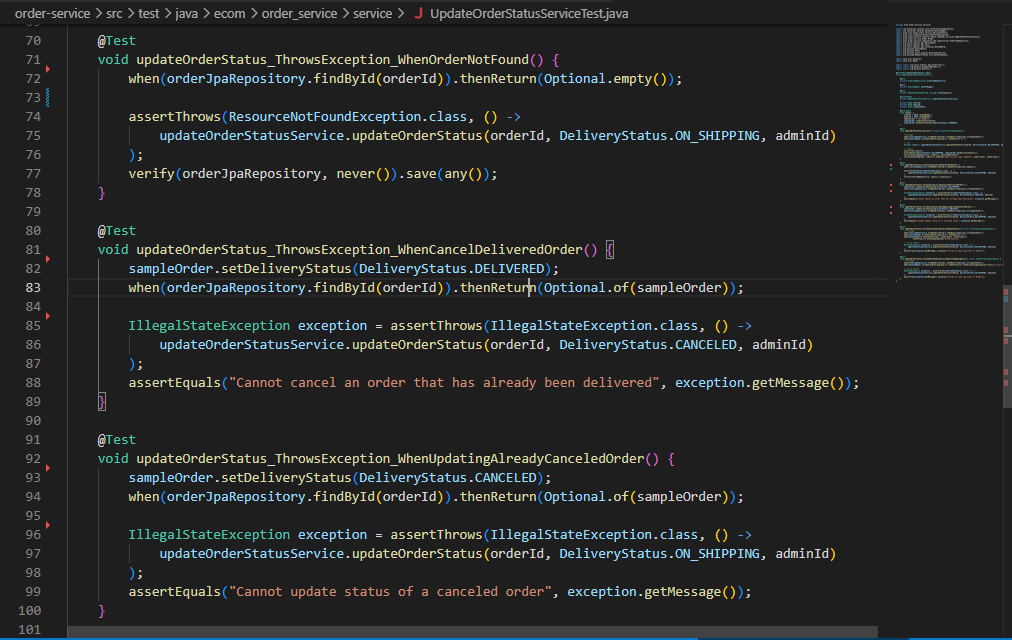
\includegraphics[width=0.9\linewidth]{images/chap8/exception_1.PNG}

\vspace{0.7cm}

\caption{Các kịch bản kiểm thử xử lý ngoại lệ trong UpdateOrderStatusServiceTest}

\label{fig:exception-order}

\end{figure}

Hình \ref{fig:exception-order} minh họa các bài kiểm thử ngoại lệ cho dịch vụ cập nhật trạng thái đơn hàng. Các kịch bản này tập trung vào việc bảo vệ tính toàn vẹn của luồng nghiệp vụ thông qua việc kiểm soát chặt chẽ các trạng thái đơn hàng.

Cụ thể, kịch bản \texttt{updateOrderStatus\_ThrowsException} xác nhận hệ thống ném ra đúng các ngoại lệ \texttt{ResourceNotFoundException} khi không tìm thấy đơn hàng, hoặc \texttt{IllegalStateException} khi vi phạm quy tắc chuyển đổi trạng thái. Các "chốt chặn" logic này đảm bảo những đơn hàng đã giao (\texttt{DELIVERED}) không thể bị hủy và đơn hàng đã hủy (\texttt{CANCELED}) không thể tiếp tục vận chuyển trái phép. Thông qua việc kiểm chứng các thông báo lỗi cụ thể bằng \texttt{assertThrows}, nhóm khẳng định hệ thống luôn vận hành ổn định và ngăn chặn hiệu quả các thao tác sai sót từ phía quản trị viên.

\subsubsection{D. Tổng hợp và thống kê kết quả kiểm thử đơn vị}

Bảng \ref{tab:full-unit-test-report} dưới đây là bảng thống kê tóm tắt kết quả Unit Testing cho các module cốt lõi:

\begin{table}[H]
\centering
\small
\begin{tabular}{|c|l|l|c|c|c|}
\hline
\textbf{STT} & \textbf{Dịch vụ} & \textbf{Tính năng} & \textbf{Pass} & \textbf{Fail} & \textbf{Tổng} \\ \hline

\multirow{3}{*}{1} & \multirow{3}{*}{User service} & Quên mật khẩu & 5 & 0 & 5 \\ \cline{3-6} 
 & & Đăng nhập & 9 & 0 & 9 \\ \cline{3-6} 
 & & \textbf{Tổng cộng User service} & \textbf{14} & \textbf{0} & \textbf{14} \\ \hline

\multirow{4}{*}{2} & \multirow{4}{*}{Product service} & Truy vấn và lọc sản phẩm & 17 & 0 & 17 \\ \cline{3-6} 
 & & Quản lý tồn kho & 11 & 0 & 11 \\ \cline{3-6} 
 & & Quản lý mã giảm giá & 5 & 0 & 5 \\ \cline{3-6} 
 & & \textbf{Tổng cộng Product service} & \textbf{33} & \textbf{0} & \textbf{33} \\ \hline

\multirow{4}{*}{3} & \multirow{4}{*}{Cart service} & Thay đổi số lượng sản phẩm & 14 & 0 & 14 \\ \cline{3-6} 
 & & Tính toán giá và giảm giá & 6 & 0 & 6 \\ \cline{3-6} 
 & & Quản lý mục trong giỏ hàng & 6 & 0 & 6 \\ \cline{3-6} 
 & & \textbf{Tổng cộng Cart service} & \textbf{26} & \textbf{0} & \textbf{26} \\ \hline

\multirow{4}{*}{4} & \multirow{4}{*}{Order service} & Truy vấn báo cáo và phí vận chuyển & 10 & 0 & 10 \\ \cline{3-6} 
 & & Quản lý trạng thái và hủy đơn & 11 & 0 & 11 \\ \cline{3-6} 
 & & Thanh toán và Đánh giá & 9 & 0 & 9 \\ \cline{3-6} 
 & & \textbf{Tổng cộng Order service} & \textbf{30} & \textbf{0} & \textbf{30} \\ \hline

\multirow{3}{*}{5} & \multirow{3}{*}{Orchestration service} & Điều phối giao dịch phân tán (Saga) & 11 & 0 & 11 \\ \cline{3-6} 
 & & Xử lý xem trước và xác nhận thanh toán & 10 & 0 & 10 \\ \cline{3-6} 
 & & \textbf{Tổng cộng Orchestration service} & \textbf{21} & \textbf{0} & \textbf{21} \\ \hline

\multirow{3}{*}{6} & \multirow{3}{*}{Admin service} & Khởi tạo dữ liệu báo cáo & 4 & 0 & 4 \\ \cline{3-6} 
 & & Kết xuất và xử lý báo cáo (Report) & 3 & 0 & 3 \\ \cline{3-6} 
 & & \textbf{Tổng cộng Admin service} & \textbf{7} & \textbf{0} & \textbf{7} \\ \hline

\multicolumn{3}{|c|}{\textbf{TỔNG CỘNG HỆ THỐNG}} & \textbf{131} & \textbf{0} & \textbf{131} \\ \hline

\end{tabular}
\caption{Thống kê chi tiết kết quả Unit Testing toàn bộ hệ thống Backend}
\label{tab:full-unit-test-report}
\end{table}